\documentclass{article}

\usepackage{fullpage}
\usepackage{amsmath}
\usepackage{graphicx}

\begin{document}

\title{Analytic Results on Bistable Schlogl Reaction-Diffusion System}
\author{}
\date{}
\maketitle

\section{System}
The reaction-diffusion system is written as
\begin{equation}
\label{reactdiff}
\frac{\partial}{\partial t}n(x,t)=D\frac{\partial^2 n}{\partial x^2}+f(n),
\end{equation}
where $D$ is the diffusion coefficient and $f(n)$ is the reaction term.
For the Schlogl model, $f(n)$ is a cubic function.
If $f(n)$ has two stable equilibrium states, it can be written as
\begin{equation}
f(n)=-k(n-n_0)(n-n_*)(n-n_+),
\end{equation}
where $n_0$ and $n_+$ are the 0 and + stable states, respectively, and $n_*$ is the unstable state.
Hence, rather than specifying the rate constants of the four reactions in the Schlogl model, we introduce the positions of the three equilibrium states, $n_0$, $n_*$, and $n_+$, and the overall rate constant $k$.
Of the two possibilities for the order of the states, we choose
\begin{equation}
n_0<n_*<n_+.
\end{equation}
For $k>0$, this holds if and only if
\begin{equation}
\int_{n_0}^{n_+} f(n)dn>0 \iff \frac{n_0+n_+}{2}>n_*.
\end{equation}

By introducing the following scaling
\begin{equation}
n(x,t)=\tilde{n}\left(\sqrt{\frac{k}{D}}x,kt\right),
\end{equation}
we can normalize Eq.~\eqref{reactdiff} as follows:
\begin{equation}
\frac{\partial}{\partial t}\tilde{n}(x,t)
=\frac{\partial^2\tilde{n}}{\partial x^2}
-(\tilde{n}-n_0)(\tilde{n}-n_*)(\tilde{n}-n_+).
\end{equation}
Hence, all physical quantities to be discussed in the subsequent sections are expressed in terms of $n_0$, $n_*$, and $n_+$ with scaling factors expressed in terms of $k$ and $D$.

\section{ODEs for Propagating Fronts}

We consider two types of propagating fronts.
The first type is the one moving in one direction and the other is the one propagating spherically.
For the first type, analytic expressions for the shape of the front as well as the propagting speed are known.
For the spherical wave, a differential equation for the shape of the critical bubble is known.

\subsection{Front Propagating in One Direction}

From the observation that the front moves at a constant speed, denoted by $c$, we introduce $n(x,t)=n(\xi)$ with $\xi=x-ct$.
Then, Eq.~\eqref{reactdiff} becomes the following ODE:
\begin{equation}
\label{frontx}
Dn''+cn'+f(n)=0.
\end{equation}
Boundary conditions at the infinities are give as follows:
\begin{equation}
\label{bc_frontx}
\lim_{\xi\rightarrow -\infty}n(\xi)=n_+,\quad
\lim_{\xi\rightarrow \infty}n(\xi)=n_0.
\end{equation}
Note that the value of $c$ also needs to be determined when Eq.~\eqref{frontx} is solved.
Also, note that there is a unique value of $c$, but there are infinitely many solutions for $n(\xi)$; if $n(\xi)$ is a solution, then so is $n(\xi+\xi')$ for any constant $\xi'$.
So, we also impose the following condition:
\begin{equation}
n(0)=\frac{n_0+n_+}{2}.
\end{equation}
Then, $c$ and $n(\xi)$ are uniquely determined as follows:
\begin{align}
\label{cprop}
& c = \sqrt{2kD}\left(\frac{n_0+n_+}{2}-n_*\right),\\
\label{nxi}
& n(\xi)=n_0+\frac{n_+-n_0}{1+\exp\Big(\sqrt{\frac{k}{2D}}(n_+-n_0)\xi\Big)}.
\end{align}
Note that while the shape of the front $n(\xi)$ does not depend on the position of the unstable point $n_*$, the propagating speed $c$ does; as $n_*$ approaches the midpoint of $n_0$ and $n_+$ from the right, $c$ decreases to zero.

\subsection{Critical Bubble for Spherically Propagating Front}

It is known that there is a threshold above which a spherically symmetric initial condtion generates a propagating wave.
We call the shape of this threshold function as the critical bubble.
The threshold function is an (unstable) equilibrium solution of Eq.~\eqref{reactdiff} (i.e., $\partial n /\partial t=0$).
Since the solution is spherically symmetric, the differential equation for $n=n(r)$ is written as follows:
\begin{equation}
D\left[n''+\frac{d-1}{r}n'\right]+f(n)=0,
\end{equation}
where $d$ is the dimensionality of the space ($d=1,2,3,\dots$).
Note that the terms in the square brackets constitute the Laplacian for a spherically symmetric function.
While $n(0)$ needs to be determined, the following conditions should hold for $n(r)$:
\begin{equation}
n'(0)=0,\quad\lim_{r\rightarrow\infty}n(r)=n_0.
\end{equation}
There is a unique value of $n(0)>n_*$ that allows a solution and $n(r)$ is uniquely determined.

\section{Observations in Phase Space}

As mentioned in the previous section, analytic expressions are known for the front moving in one direction, whereas no analytic expressions are available for the spherically propagating wave.
In this section, we compare the solutions of the two cases in the phase space.
In other words, for a solution $n=n(\xi)$ or $n(r)$, we define $u(t)\equiv n(t)$ and $v(t)\equiv n'(t)$ and plot $(u(t),v(t))$. 
Note that although $n$ is a function of $\xi$ or $r$, we interpret it as a function of $t$ in this section.
We show that, in the phase space, the solution of the former case is very similar to that of the latter case for two or higher dimensions.
From this, we will deduce an approximate expression for the size of the critical bubble for $d>1$ in the next section.

We begin with writing down vector field equations that each solution satisfies: 
for the one-direction propagating wave, 
\begin{equation}
\label{vf_x}
\begin{split}
&\dot{u}=v,\\
&\dot{v}=-\frac{f(u)}{D}-\frac{c}{D}v;
\end{split}
\end{equation}
and for the spherically propagating wave in the $d$-dimensional space,
\begin{equation}
\label{vf_sph}
\begin{split}
&\dot{u}=v,\\
&\dot{v}=-\frac{f(u)}{D}-\frac{d-1}{t}v.
\end{split}
\end{equation}
Note that $c$ is unknown in Eq.~\eqref{vf_x}, whereas the vector field given in Eq.~\eqref{vf_sph} is time-dependent.
To understand these complicated vector fields, we introduce the following time-independent vector field:
\begin{equation}
\label{vf_0}
\begin{split}
&\dot{u}=v,\\
&\dot{v}=-\frac{f(u)}{D}.
\end{split}
\end{equation}
In the left panel of Fig.~\ref{fig_vf_b1_p}, the vector field around the three equilibrium points $(n_0,0)$, $(n_*,0)$, and $(n_+,0)$ is shown.
It can be seen that $(n_0,0)$ has a homoclinic orbit (enclosing the point $(n_*,0)$) but $(n_+,0)$ does not.

\begin{figure}
\centering
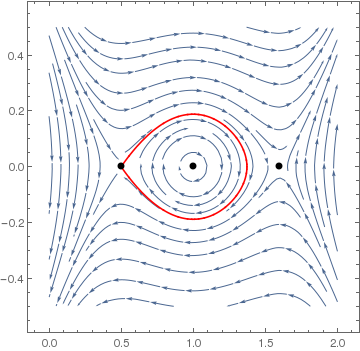
\includegraphics[width=0.3\linewidth]{fig1/vector_field_b1.png}
\hspace{5mm}
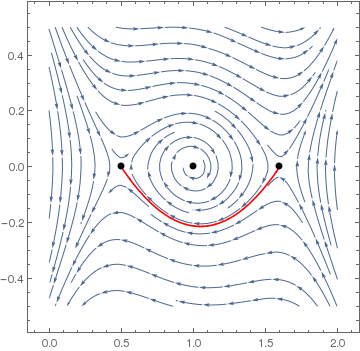
\includegraphics[width=0.3\linewidth]{fig1/vector_field_p.png}
\caption{\label{fig_vf_b1_p}(Left) The vector field given in Eq.~\eqref{vf_0} and the homoclinic orbit of $(n_0,0)$ are plotted. This vector field corresponds to the one-dimensional critical bubble case. (Right) The vector field given in Eq.~\eqref{vf_x} with $c$ defined in Eq.~\eqref{cprop} is plotted. The heteroclinic orbit from $(n_+,0)$ to $(n_0,0)$ is also plotted. This vector field corresponds to the one-direction propagating front case. The following values are used: $n_0=0.5$, $n_*=1$, $n_+=1.6$, $k=D=1$.}
\end{figure}

\begin{figure}
\centering
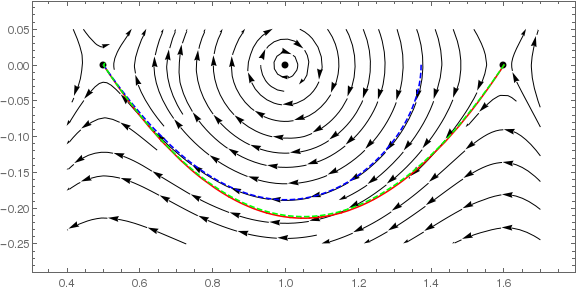
\includegraphics[width=0.5\linewidth]{fig1/vector_field_half.png}
\caption{\label{fig_vf_half}On the vector field given in Eq.~\eqref{vf_0}, the solutions of the one-direction propagating wave (by the red solid line) and the one- and two-dimensional critical bubbles (by the blue and green dotted lines, respectively) are plotted. The following values are used: $n_0=0.5$, $n_*=1$, $n_+=1.6$, $k=D=1$.}
\end{figure}

Now we compare the solutions by plotting them in the phase space, see Fig.~\ref{fig_vf_half}.
We first look at the trajectories of the one-dimensional critical bubble $n_\mathrm{b1}(r)$ and the one-direction propagating wave solution $n_\mathrm{p}(\xi)$.
Since Eq.~\eqref{vf_sph} reduces to Eq.~\eqref{vf_0} for $d=1$, the trajectory of $n_\mathrm{b1}(r)$ in the phase space is nothing but one half of the homoclinic orbit of $(n_0,0)$ with $v<0$, see the left panel of Fig.~\ref{fig_vf_b1_p}.
On the other hand, the trajectory of $n_\mathrm{p}(\xi)$ can be drawn in the phase space from its analytic expression given in Eq.~\eqref{nxi};
we can show that its trajectory is expressed as
\begin{equation}
v= \sqrt{\frac{k}{2D}}(u-n_0)(u-n_+)\quad(n_0\le u\le n_+).
\end{equation}
In fact, this trajectory is the heteroclinic orbit from $(n_+,0)$ to $(n_0,0)$ of the vector field given in Eq.~\eqref{vf_x}, see the right panel of Fig.~\ref{fig_vf_b1_p}.
The difference between the two trajectories in the phase space can be understood by the difference between the vector fields given in Eqs.~\eqref{vf_x} and \eqref{vf_0}.
Due to the additional term $-\frac{c}{D}v$ in Eq.~\eqref{vf_0}, the starting point $(n_\mathrm{p}(0),0)$ should be further away from $(n_0,0)$ than $(n_\mathrm{b1}(0),0)$.

Finally, we consider the critical bubble of two- or higher-dimensional cases.
As shown in Fig.~\ref{fig_vf_half} for the two-dimensional case, the trajectory of $n_\mathrm{b2}(r)$ is different from that of $n_\mathrm{b1}(r)$. 
This is quite expected because the additional term $-\frac{d-1}{t}v$ becomes nonzero for $d\ge2$.
More interestingly, however, the trajectory of $n_\mathrm{b2}(r)$ is very close to that of $n_\mathrm{p}(\xi)$.
This behavior is also observed for the three dimensional case and the closeness of the two trajectory becomes even better.

\section{Approximate Expression for the Critical Bubble Size} 

In the previous section, we have observed that the trajectory of the critical bubble for $d\ge2$ in the phase space is very similar to that of the one-direction propagating wave. Now we closely look at the two cases and deduce the critical bubble size $R_d$ from the propagation speed $c$ of the one-directional wave.

The trajectory of the one-direction propagating front in the phase space can be described as follows.
Although it takes infinite time for the trajectory to leaving the starting point $(n_+,0)$, once it leaves the neighborhood of the point, it moves quickly into the neighborhood of $(n_0,0)$.
Then, the trajectory spends infinite time approaching the point $(n_0,0)$.
On the other hand, the trajectory of the critical bubble for $d\ge2$ in the phase space can be described as follows.
Since the starting point is very close to $(n_+,0)$, the trajectory spends plenty of time near $(n_+,0)$.
Once it leaves the neighborhood of $(n_+,0)$, it moves quickly into the neighborhood of $(n_0,0)$.
Then, the trajectory spends infinite time approaching $(n_0,0)$. 

Based on the closeness of the two trajectories, it is expected that the two vector fields are similar when the two trajectories quickly move from the neighborhood of $(n_+,0)$ to that of $(n_0,0)$. 
Hence, the additional terms in the two vector fields, which are $-\frac{c}{D}v$ and $-\frac{d-1}{t}v$, should be similar.
On the other hand, when the trajectory of the critical bubble in the phase space quickly moves, the value of the solution $n(r)$ quickly changes.
Hence, if we denote the critical bubble size by $R_d$, the value of $t$ in the additional term $-\frac{d-1}{t}v$ can be approximated by $R_d$.
Then, by equating the two terms, we finally obtain
\begin{equation}
\label{Rd}
R_d\approx\frac{(d-1)D}{c}.
\end{equation}
By substituting the analytic expression of $c$ in Eq.~\eqref{cprop}, we obtain
\begin{equation}
\label{Rd_full}
R_d\approx (d-1)\sqrt{\frac{D}{2k}}\left(\frac{n_0+n_+}{2}-n_*\right)^{-1}.
\end{equation}

In order to test the validity of Eq.~\eqref{Rd_full}, we compare the profile of the critical bubble solution ($d=2$ and 3) with that of the \textit{translated} one-direction propagating front solution $n_p(r-R_d)$.
As shown in Fig.~\ref{fig_comp_prop_bubble}, the agreement is remarkably good for the parameter values $n_0=0.5$, $n_*=1$, $n_+=1.6$, $k=D=1$.
 
\begin{figure}
\centering
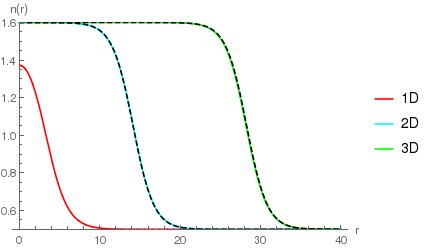
\includegraphics[width=0.5\linewidth]{fig1/comp_prop_bubble.png}
\caption{\label{fig_comp_prop_bubble}The profiles of the critical bubbles for $d=1,2,3$ are plotted. In addition, the profiles of the one-direction propagating fonts translated by $R_d$ ($d=2,3$) are also plotted for comparison.}
\end{figure}

\end{document}
